\documentclass{ltjsbook}
\usepackage{docmute} 
\usepackage{../../myStyle} 

\begin{document}
\setcounter{chapter}{10}
\chapter{システム論からみた社会心理学：第五世代システム}
\label{sp11_system}

\section{第四世代システムのまとめ}
それでは，時間にもなりましたし，お客さんもいらっしゃいましたので，お話を始めようかなと思います。今回と，あと1回，計2授業があります。それでおしまいということになります。

授業としては，3部作のその2が今日で終わるので，最後の1回だけでその3をしないといけないんですけれども，コンパクトにまとめて何とかしようと思います。今日中にこの第2部のパートは確実に終わらせて，可能なら第3部の頭のところぐらいを触れられたらな，というふうに思いつつ始めていきたいと思います。

第2部ということで，システム論から見た社会心理学という話をずっとやっているわけですが，前回は第四世代システム\index[termidx]{だいよんせだいしすてむ@第四世代システム}というお話をしました。複雑系\index[termidx]{ふくざつけい@複雑系}，コンプレックスシステム\index[termidx]{こんぷれっくすしすてむ@コンプレックスシステム}ですね。第四世代システム\index[termidx]{だいよんせだいしすてむ@第四世代システム}の特徴というのは，基本的にはエージェントがシンプルな動作しかしていないんだけれども，そこから複雑な現象が創発\index[termidx]{そうはつ@創発}するというのがテーマのシステム論でした。

このエージェントが分散的に，別々に自分の振る舞いをしていて，しかもそれが局所的に相互作用する。あちこちで同じようなルールのエージェントが，相互作用するというそれだけのルールで，非常に複雑な振舞が表面的に全体的に現れるというのが，コンプレックスシステム\index[termidx]{こんぷれっくすしすてむ@コンプレックスシステム}の特徴というお話をさせていただきました。

システム論として複雑系\index[termidx]{ふくざつけい@複雑系}を見るときの特徴は何だったかといいますと，一つは最初からパターンのシステムになっていたということですね。物理的実体を持ったシステムではなくて，それっぽく見えるパターン，複雑に見えるという見え方でシステムだと呼んでいるということです。それが，パターンの見え方，もちろん物理的な実体というのがベースにはなっているのですが，それに基づく全体的なパターンというのがシステムとして考えるものなのだとしているところが，一つのポイントです。

もう一つは局所的相互作用\index[termidx]{きょくしょてきそうごさよう@局所的相互作用}，近傍の概念ですね。セルオートマトン\index[termidx]{せるおーとまとん@セルオートマトン}やライフゲームを見ていただきましたが，自分の周囲とだけ相互作用している。全体のことが分かっているわけではないんです。そういう状態なんだけれども，全体のレベルでは複雑なパターンが出てきていると。

ライフゲームの中では，画面の左上から右下の方に，4回パターンを変えて移動するグライダー\index[termidx]{ぐらいだー@グライダー}という形をご紹介したかと思いますが，あのグライダー\index[termidx]{ぐらいだー@グライダー}というのは，1個1個のセルが自分がグライダー\index[termidx]{ぐらいだー@グライダー}の要素を作っているという自覚はもちろんないわけです。それぞれのセルは，自分と周囲のパターンを見て，次のターンに自分がオンになるのかオフになるのかを決めているだけです。

それぞれの要素が重なり合っているというところはあるのですが，全体のうちどのくらい自分の要素を参照しているかという，全体と自分の周囲との参照の比率が全体のパターンを作っているのに関係がありそうだということが見えてきますね。これにしても，移動空間上の周りのセルとのネットワークが中心にキーになっているというところは知っておいてください。

生き物のように見える複雑系\index[termidx]{ふくざつけい@複雑系}，複雑なパターンというのは，成長する，再生する，増殖するというものが主です。それらの特徴で持って，生きているもののように見える，生き物のように見えるということを表現しています。それまでのシステム論と大きく違うところは，一つは最初から一つ一つのセルが「独立したシステムになっているわけではない」ということです。オートポイエーシス\index[termidx]{おーとぽいえーしす@オートポイエーシス}は，システムの個体性を重視します。生命はそれだけで完全な1個体なのだ，というところが特徴です。しかしそういった前提を置いたら，複数のシステムがある場合にはどうするのか。また，自分というシステムと，自分以外というシステムとの関わり方はどうなるのか，といったことについては，「構造的にカップリング\index[termidx]{かっぷりんぐ@カップリング}している」というのに止まっています。

複雑系\index[termidx]{ふくざつけい@複雑系}に対しては，それぞれのシステムがそのシステムと周辺の近状に存在する他のシステムと関わっているという点で，最初から複数のシステムが繋がっていることを前提にしています。この考え方がシステム論としては新しいところかもしれません。

これらを踏まえて，社会心理学的にシステム論を考えていく方向に進んでいく必要があります。複雑系\index[termidx]{ふくざつけい@複雑系}は，「複雑適応系」という言い方もあります。エージェントは環境の複雑さを反映しているだけで，エージェント自身はそれほど複雑なルールを持っていないという考え方もあるのですが，それでも問題はないと思います。

しかし，それぞれのシステムが何を目指しているのか。特にパターンが現れるとき，それを構成するシステムとどういう関係にあるのか，という関係性はどうなっているのでしょうか。複雑系\index[termidx]{ふくざつけい@複雑系}は全体主義的なところがあり，全体を見てパターンを見つけるのみで，そのパターンを見ている者は誰なのか，それぞれのシステムの目的関数はどうなっているのかということについては明らかにされていません。

これを踏まえて，今日は「第五世代のシステム論」に進みたいと思います。第五世代のシステム論は，「複合システムネットワーク\index[termidx]{ふくごうしすてむねっとわーく@複合システムネットワーク}論」を元にお話ししていきたいと思います。藤澤等\index[nameidx]{ふじさわひとし@藤澤等}という関西大学に長らくお勤めだった先生が提唱した理論です。

\subsection{第五世代システム論へ}

今お見せしているテキスト，「複合システムネットワーク\index[termidx]{ふくごうしすてむねっとわーく@複合システムネットワーク}論」\parencite{fujisawaNetwork}は，実は3部作のうちの1つで，さらに第4巻，第5巻まで出る予定だったシリーズの一部です。0，1，2とありますが，0巻が「ソシオン\index[termidx]{そしおん@ソシオン}理論のコア」\parencite{fujisawaCore}というタイトルがついています。そして，2巻目がシリーズナンバー1で，「複合システムネットワーク\index[termidx]{ふくごうしすてむねっとわーく@複合システムネットワーク}論」\parencite{fujisawaNetwork}です。これが純粋なシステム論の話をしているところです。

3巻目には「関係科学への道」があり\parencite{fujisawaRelationships}，4巻目には「社会-心理学」の本が予定されていましたが，実際に出版されたのは冒頭の3巻だけでした。このシリーズの2巻目を中心に，今日はお話をしていきたいと思います。

これは私の学部時代の恩師である，藤澤等\index[nameidx]{ふじさわひとし@藤澤等}が考えたシステム論です。この後のシステム論，新しい見方というのは私は詳しく知りませんが，それまでのシステム論が生物学，化学，神経科学，情報科学から来ていたのに対して，社会心理学でのシステム論，自分の社会科学を経営におけるシステム論という意味では非常に新しいのではないかと思いますので，ぜひ紹介していきたいと思います。


\section{第五世代システム論の特徴}
\subsection{ネットワークというアプローチ}

さて，複合システムネットワーク\index[termidx]{ふくごうしすてむねっとわーく@複合システムネットワーク}論というタイトルにありますように，いくつか既にキーワードがあります。まずは「複合」ですね。そのまま単一のシステムを扱うものではないということ，オートポイエシスのように，1生命1個体を扱うものではないと。複数のシステムを最初から見据えてあるというところがポイント1です。

その次に複合システム\index[termidx]{ふくごうしすてむ@複合システム}のネットワーク論ということで，ネットワークになっているということですね。このネットワークになっていることからわかるように，複雑系\index[termidx]{ふくざつけい@複雑系}の要素が入っていますね。もっとも，社会心理学においてネットワークという発想はもう当然のように昔からありまして，対人関係のネットワークとか，対人援助のネットワークみたいな言い方もされたりするわけです。

さらに古くは，レヴィン\index[nameidx]{れゔぃん@レヴィン}のライフスペースという話があったかと思います。(図を黒板に描きながら)A,B,C,D,E...と，いくつかの要素がこのように生活空間といわれる空間の中にあるというやつですね。レヴィン\index[nameidx]{れゔぃん@レヴィン}が考えたライフスペース(生活空間)というのは，ある一時点を切り取ったときの集団全体に影響を与える場，フィールドとして描かれているのでしたね。

そのときのここの要素が一人一人の人間であってもよいし，そこに物理的な実態として存在するわけではない実体でもいいんです。客観的に実在するのはいいんですが，物理的な実態から外れた，しかしその心理的な変化に影響を与える社会的な実在，認知的な要素などをも含めた，その場に影響する全体が含まれているのがライフスペース。さらに，レヴィン\index[nameidx]{れゔぃん@レヴィン}は，ある時点から次の時点への変化を考える学論として，集団における社会科学におけるフィールドセオリー(場の理論)を考えたわけですね。

\begin{figure}[ht]
	\centering
	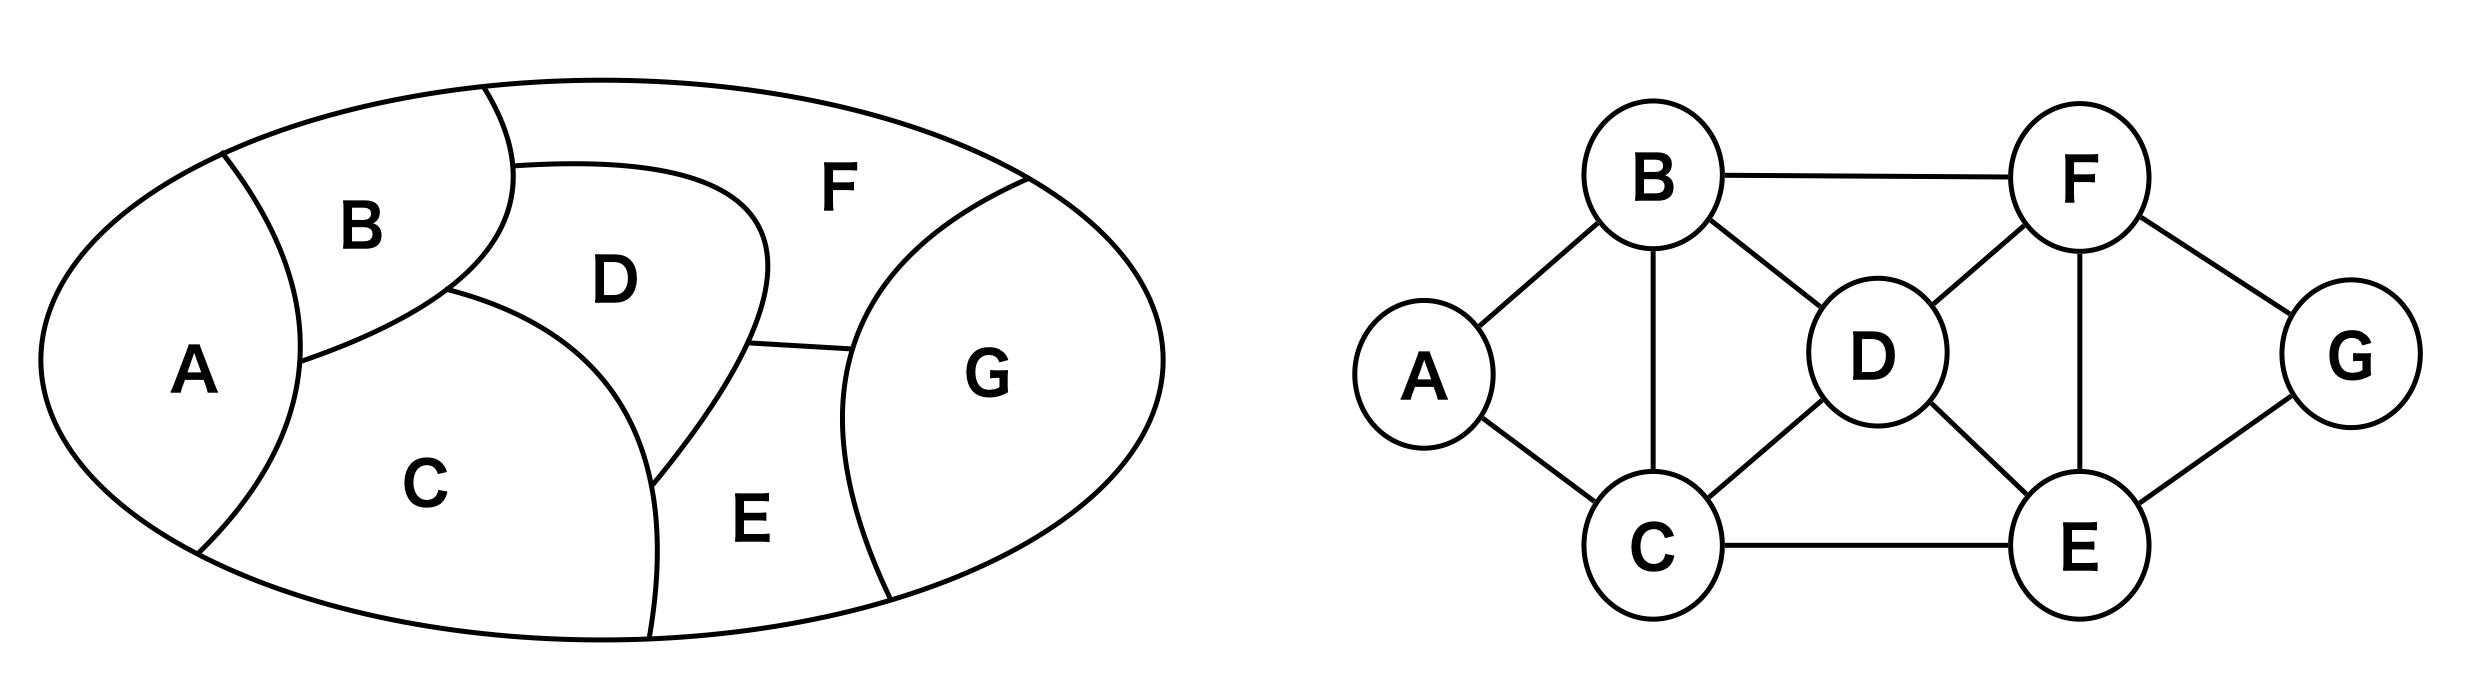
\includegraphics[keepaspectratio,width=0.7\linewidth]{../images/11_LewinNet.png}
	\caption{レヴィン\index[nameidx]{れゔぃん@レヴィン}の生活空間。鱗状の表現(左)とネットワーク表現(右)は等価}
	\label{LewinNet}
\end{figure}

この場の変化量を考えるからダイナミクスなんだ，という話をしたわけですが，実はこのライフスペースという表現で重要なのは，例えば今私がここに描いた絵でいうと，要素AがBとかCとかと接しているんだけれども，Dとは接していないというところですね。で，これ(図 \ref{LewinNet}左)は鱗状の図では書いてあるんですけれども，これを別の描き方をすると，ネットワークのような図になります。AはB,Cとつながっている，BはC,D,Fとつながっている，FはB,D,E,Gとつながっている，というようにね。こういうふうに要素同士がどことつながっているかということが重要だということを論じていたわけです。レヴィン\index[nameidx]{れゔぃん@レヴィン}は鱗状の形で描いてますが，ここの面積が重要だという話はしておりません。力が伝播する経路が大事なんだという形で，このライフスペースを描いているわけですね。

どことどこがつながっているかというのをトポロジーと言いますが，その位相的な関係をレヴィン\index[nameidx]{れゔぃん@レヴィン}は描きたかったわけです。という意味では，こっち(図 \ref{LewinNet}右)に書いてあるような要素と線で描いているようなネットワークの図と同じことを別の表現していたわけでして，レヴィン\index[nameidx]{れゔぃん@レヴィン}もこうやってネットワークのことを考えていたわけですね。


社会科学における人間関係のネットワークという時は，誰と誰が友達ですか，連絡帳に名前が相互に載っているのは誰と誰ですかというような形で操作的に定義して使ったりします。その社会的なつながりを変数として研究するわけですが，それよりもずっと前にレヴィン\index[nameidx]{れゔぃん@レヴィン}は同じくネットワーク構造とについて考えていたわけです。

\subsection{ネットワークの理論の系譜}

ちなみに，このネットワークの理論そのもののスタートは，数学においてオイラーが始めたケーニヒスベルグの橋問題です\footnote{ケーニヒスベルクの橋の問題は，18世紀のプロイセン王国ケーニヒスベルク(現ロシア・カリーニングラード)に実在した7つの橋を一度ずつ渡り，元の場所に戻ることができるかという問いです。数学者レオンハルト・オイラーは，この問題を抽象化し，グラフ理論の概念を用いて解決しました。彼は，全ての辺を一度だけ通る閉路(オイラー閉路)を持つグラフは，全ての頂点の次数が偶数であることが必要であると示しました。ケーニヒスベルクの橋の問題に対応するグラフでは，全ての頂点の次数が奇数であったため，オイラー閉路は存在せず，一度ずつ全ての橋を渡ることは不可能であると結論付けられました。この研究は，グラフ理論の発展に大きく寄与しました。(Wikipediaより)}。
彼が住んでいた町に何かいくつか橋がかかっているんだけれども，それを散歩する時に全部一筆書きで通ることはできるか，できないか，というパズルを考えていたことが発端です。どのエリアとどのエリアがつながっているか，どうつながっているか，というつながりだけの関係を考える数学ということで，トポロジー，位相数学，グラフ理論というのが出てきています。

数学的にはそのようにして考えられ始められました。ネットワーク論としては，ネットワークの一個一個の結び目のことをノード\index[termidx]{のーど@ノード}nodeと言います。また，この結び目と結び目をつなぐ線のことを紐帯\index[termidx]{ちゅうたい@紐帯}tieとかエッジ\index[termidx]{えっじ@エッジ}edgeと呼ぶことになってます。このつながり方の科学というのを考えたところから，ネットワークモデル，グラフ理論が始まり，数理社会学のほうでは社会ネットワーク論として応用されています。もちろん，数学的な方向でもいろいろ発展しているので，興味がある人は調べていただければと思います。ともかく，このようなものとしてどことどこがどうつながっているか，そのネットワークの振る舞いというのを研究する領域というのがございます。

\begin{figure}[ht]
	\centering
	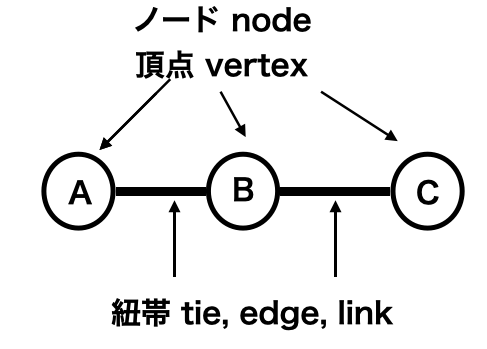
\includegraphics[keepaspectratio,width=0.3\linewidth]{../images/11_network_words.png}
	\caption{ネットワークモデル，グラフ理論の用語}
	\label{network}
\end{figure}

ちなみにネットワークモデルが面白くなるのは，レヴィン\index[nameidx]{れゔぃん@レヴィン}のこの鱗状の図の時に説明したかと思いますが，単純に2つのものがつながっているだけではだめなんですね。例えば要素がAとBだけでつながってます，というだけだったらハイそうでうすね，で終わるんです。ネットワークがネットワークとしての特徴を見せるのは，自分が直接つながっていないノード\index[termidx]{のーど@ノード}との関係を見る時です。例えばこの横一長線の図のようにA，B，Cとあったとします。ここでAはBとはつながっていますが，Cとはつながっていないんですね。つながっていないんですが，AがBに与えた影響がCにも伝播するわけです。Bを経由してね。

レヴィン\index[nameidx]{れゔぃん@レヴィン}のときも触れたかと思うんですが，AがBやCに影響することがあったとして，それが何ステップか経て，最終的には直接つながっていない別の要素にも影響を与えるんだよという，ところが面白ポイントです。これでネットが初めてワークするんです。しかも，そのルートが左から右へ一方向ですよというのではなくて，何らかの形でフィードバックが返ってくるときです。

たとえば図\ref{loop}のように，AがBに，BがCに，CがBにしてAにその影響が戻ってくるというような，誰か第三者ですとか，他のものを介して影響が自分のところに返ってくるというようなことがあれば，ネットワークが独特の振る舞いをし始めます。

\begin{figure}[ht]
	\centering
	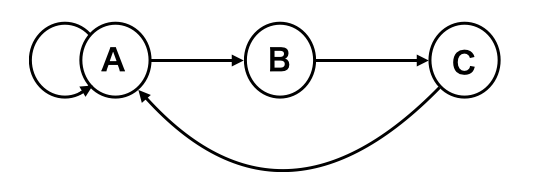
\includegraphics[keepaspectratio,width=0.5\linewidth]{../images/11_Loop.png}
	\caption{フィードバック，自己回帰などのループが複雑さを増す}
	\label{loop}
\end{figure}

そういう直接自分とは関係のないものと繋がっていること，自分の発した情報なり，影響力というのが巡り巡って自分の状態に影響を与えること，このあたりがネットワークがネットワークとして面白くなるところです。さらに加えて，第二世代の自己組織化系\index[termidx]{じこそしきかけい@自己組織化系}のように，「自分の反応が自分に影響する」ということも当然考えられるわけで，こういった自分に対する再起的な影響力を考えますと，ネットワークの振る舞いは非常に複雑なものになります(図\ref{loop}のAのループを描きながら)。

第二世代システム\index[termidx]{だいにせだいしすてむ@第二世代システム}は自己組織化系\index[termidx]{じこそしきかけい@自己組織化系}ということで，$t$時点の自分の状態が$t+1$時点の自分の状態に影響しているという話をし余した。これって，自分に帰ってくるループがあるということですもんね。しかもそれが微分系ではなくて差分系で書かれているというのが，第二世代としての特徴だったわけです。このフィードバックと差分システムにすることによって自己組織化系\index[termidx]{じこそしきかけい@自己組織化系}というのは，非平衡的な状態から突然考えられないような状態に相転移\index[termidx]{そうてんい@相転移}する。急に状況が変わるというようなジャンプを生み出すわけですが，この源泉が自己回帰ループにあります。

\section{ 藤澤の複合システムネットワーク論}

\subsection{社会心理学的なネットワークの単位}
ということで，社会心理学において，要素同士のネットワークというのを中心にシステム論を考えてみましょう。この1個1個のノード\index[termidx]{のーど@ノード}が複数あり，ネットワークを組んでいること。そして1個1個のシステムを考えるというのが，今回の複合システム\index[termidx]{ふくごうしすてむ@複合システム}のネットワーク論ということです。オートポイエシスのように単体ではなく，複合的なことを考えること。自己組織化系\index[termidx]{じこそしきかけい@自己組織化系}のときのように差分方程式，あるいは自己回帰的な自分に帰ってくるようなものを考えること。複雑系\index[termidx]{ふくざつけい@複雑系}のときのように極端な相互作用からなる全体を考えること，このあたりが，この藤澤の第五世代システム\index[termidx]{だいごせだいしすてむ@第五世代システム}論の特徴になっています。

もちろん，第三世代のオートポイエシスと，第四世代の複雑系\index[termidx]{ふくざつけい@複雑系}のときから，システム論の力点が物理的な実態に関するシステム論から，パターンですとか，機能的なつながりというところへと変わっているというか，扱う要素の対象が変わっているというところも重要です。


皆さん，社会心理学を考えるときに，社会と個人という関係の心理学だというふうにお考えになるかと思うんですが，そのときの個人というのは物理的なものかというと，そうではないですよね。皆さんが考える自分自身というのは，もちろんこの物理的な生き物としてのハードウェアの上に成立しているものですけれども，このハードウェアの中で走っているソフトウェアのほうが個人っぽいと思います。さてでは，そのソフトウェアだけかというと，そうでもないのではないかと。少なくとも物理的なものが個人なのだというようなことを社会心理学はやりたがっているのかというと，おそらく違うでしょう。なぜなら，その物理的なものを研究の対象にしているのであれば，社会はそもそも成立しないからですね。社会というのは目に見えて触れるものではないからです。

目に見えて触れるものではなくて，社会的な実在としてみんながあると考えているものが研究の対象，社会の研究対象なんだとしたら，それを構成しているであろう個人の方も物理的な存在ではなくて，何らかのパターンであるはずです。位相的なものではないといけない。つまり，我々人間一人一人の個人というのも，関係的な要素のパターンになっているというところから考えなければならないというわけですね。

さて藤澤は，社会を構成する最小単位について考えました。彼は個人や集団を含む社会全体を，レヴィン\index[nameidx]{れゔぃん@レヴィン}のライフスペースのように動的な全体として捉えています。そこで，この社会システム\index[termidx]{しゃかいしすてむ@社会システム}の基本要素として「ソシオン\index[termidx]{そしおん@ソシオン}」という概念を提案しました。これは，物理学での原子や分子のような，社会(Soci-)における最小構成単位(-on)という意味の造語です。このソシオン\index[termidx]{そしおん@ソシオン}socionを使って，個人と社会の関係をシステム的に説明しようとしたのです。

彼が考えているシステム論は，社会的なネットワークということについて考えられたものです。ただ，ちょっと注意しておいてほしいんですが，今からこの話がすごく誤解をされやすくなってくるので，注意してください。というのも，一般的にネットワークの話というときは，ノード\index[termidx]{のーど@ノード}が何かと結びついているということでそれを表現します。例えば「コンピューターネットワーク」という言い方をしたら，コンピュータAとBが電話回線などを使って通信しているということですよね。この時にパソコンA,Bがノード\index[termidx]{のーど@ノード}で電話回線がエッジ\index[termidx]{えっじ@エッジ}と呼ばれますが，この考え方では第三世代システム\index[termidx]{だいさんせだいしすてむ@第三世代システム}にすら到達していないわけです。というのも，ノード\index[termidx]{のーど@ノード}が物理的な実体になっているからです。物理的な実体のシステムを考えるのではなくて，考えるべきは人と人との「つながり」「関係性」を要素としたネットワークを考えるんですね。しかし，基本的には目に見えないつながり，あるいは，そのつながりの強さみたいなものが要素，ノード\index[termidx]{のーど@ノード}になったものとして，ネットワークを描くのです。

その点を誤解しないようにしてください。この辺が言葉ではちょっとなんといえば言いにくいところでもあるんですが，伝わっているものと信じてお話をしていきたいと思います。

\subsection{個人と社会の入れ子構造}

さて，藤澤が考える社会ネットワークシステムの最小単位というのはどういうふうになっているかというと，何かと何かをつなげるので，関係の上糸の形として丸く書いておきます。そして，これがメタファーとして言うならば社会心理学の社会の単位だから個人なんだと言いたいところですが，彼の「個人」というのはこの丸の中だけで終わるものではないので注意してください。

彼が考える社会の一番小さな構成単位はどういう形をしているかというと，こういう形をしています(図 \ref{socion})。この小さな丸は他の単位との結びつきの強さを表しています。関係の強さ，関係の濃度と考えてください。形としては何か中途半端な感じになってますけれども，正確に書くならば，こっち側に他の要素があるわけです。

\begin{figure}[ht]
	\centering
	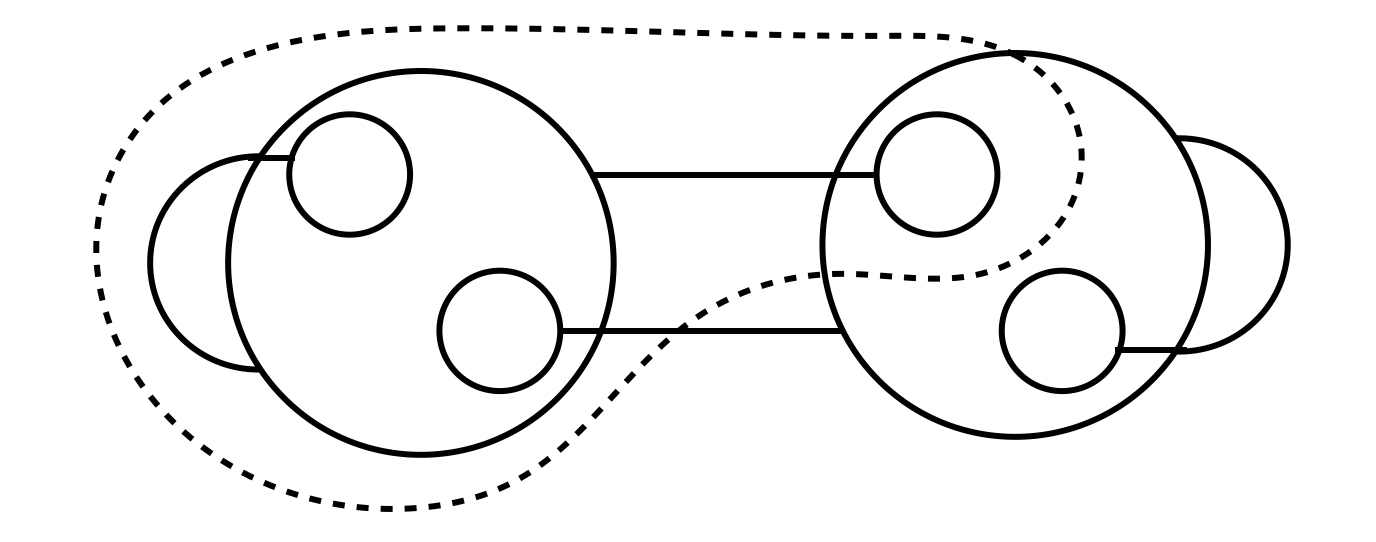
\includegraphics[keepaspectratio,width=0.7\linewidth]{../images/11_singleSOCION.png}
	\caption{社会ネットワークの最小単位}
	\label{socion}
\end{figure}

2つの要素だけからなるパターンの場合は，こういう図で書けば良いと思います。しかし，これはシステムネットワークですので，社会ネットワークということを考えますと，システムを単体で考えるときには既に他のものがないといけません。藤澤が考える一番小さな一単位というのは，この点線で囲んだところになるでしょうか。

何やら入れ子になっているので，おかしな感じを持たれるかもしれませんが，彼のアイデアの一番のポイントは，自分を形成する要素，この丸が自分だとすると，自分を形成する要素が自分の境界の外とのつながりの強さを含めて作られている，ということです。

人間で例えて考えるなら，コスギという要素を考える時，普通の人間は「あなたはどんな人間ですか？」と聞かれると，「私は私です。僕は，小杉はこういう人間です」とか，自分自身について話しますよね。でも社会的な存在としての自分を考えると，かつてジェームズが言ったように，他人の中にある自分の像もその人の一部なわけです。ですから，「私」という人間がどういう存在かというと，私を見ている人の中にも私を構成する要素があるはずです。他人の中にいる私の像は私の像であって，他人の中にありながら，自分の外縁でもあるわけです。

そういった外縁というのは，私と関わる人数と同じだけ存在するはずで，みんなの中にある私の像というのも全部，それぞれが私を構成する，「私」というネットワークの構成要素の一つだと考えます。相手が一方的に私のことを知っているだけではなく，私も相手のことを知っている。お互いに知り合っている。もちろん私にも知っている人がいっぱいいます。例えば，私とパートナーとの関係で考えると，彼女の中には私の像があるでしょう。そして，私の中には彼女の一部があるわけです。お互いに自分の存在を持ち合っているわけですね。これをどう表現するかというと，レヴィン\index[nameidx]{れゔぃん@レヴィン}のいう相互依存関係interdependencyに相当しますよね。

レヴィン\index[nameidx]{れゔぃん@レヴィン}の弟子たちがそれを間違って，自分の中にある他人に対する評価だけを切り出して，それを足し合わせて「社会」と言ってしまったのは，本来複雑に相互に依存し合っている，持ち合っている関係で初めて成り立つはずの人間関係を紐解いてしまい，足し合わせて「全体」にするという構造の形を変えちゃったところにあるのです。

本来，私と相手の関係は，相互にイメージを持ち合っていることにあるはずなんですね。私が持っている他人の像，他人の中に預けた自分の像。そういうものが色々と相互に持ち合って，繋がっているということで，そのネットワークというのが単位を構成している。1単位はどこですか？と言われると，この点線で切ったところになりますが，この単位が複数ないとネットワークにならない。少なくとも3つのtieが必要で，ここだけで成立しているわけではないということですね。そして，内部に像を含んでいる境界で持って一個人だと思いがちですが，これは必ずしも物理的な境界である必要はありません。

私たちが生きている，私たち人間，私たちの社会的な存在が生きているとはどういうことかを改めて考えてみてください。もちろん，生きているか死んでいるか，生理学的なことを考えると，瞳孔が開いていたら死んでいるとか，脈拍が止まっていたら死んでいるとかで，定義をすることができます。

しかし，社会的に生きているか，社会的に死んでしまうということがどういうことかというと，その人の名前が忘れ去られるとか，誰もその人の像のことをこの全体のネットワークの中に持っていないときではないですか。誰にも忘れ去られて，社会の中に像が残らなかった時に，初めて社会的に死ぬわけです。物理的な生命よりも社会的な生命のことを優先すること，社会的な生命が大事だという感覚は，実はよくあることです。社会的に生きるということは，その人の名前が残ることであったり，その人という社会的な実在が語られ続けていることだと考えた方がいいですよね。

ヴィトゲンシュタインは生き物としては死んでいますが，今でもあちこちで彼がどう考えたということを議論しているわけですから，社会的には彼は生きているわけです。あるいは，武士なんかは，「命を惜しむな，名をこそ惜しめ」と言いますね。生きているというのは，生物的に生きているというだけではないんですよ。この標語は，「生物的に生きているよりも，その人の名前が残っていることの方が社会的な生命としては重要なんだ」というようなことを表現しているとも言えます。何度も言うようですが，生命とは何かということを考えるのがシステム論なんですけれども，オートポイエーシス\index[termidx]{おーとぽいえーしす@オートポイエーシス}以降，物理的な生き物であるということよりは，この社会的なパターンの方が重要だということですね。

\subsection{自己の形成}

「あなたは何者ですか?」とか「自己紹介しなさい」といわれたら，「私はこういう人間ですよ」とお返事しますね。そのとき注目されているのは何かと言いますと，おそらく非常に特殊な，この自分に対する回帰的な像です。これがおそらく一般的に言われる「私個人」じゃないかと思われているようです。他人の数だけ自分がありますよ，というようなことを言うと，自我が分裂しているような気もしますけれども，この自分に対する回帰的な像はひとつしかないからです。

子どもの自我の発達過程から考えてみましょう。子どもは父親や母親から視線を向けられます。子どもは，相手の中に映る自分の像を感じ取ることができます。「大人が自分を見ているな」と。この時，複数の人から異なるタイミングで視線が送られてきます。様々な方向から来る自分に対する像には，ズレが生じます。そのような，いろんな方向から来る自分に対する像を，その齟齬・ズレみたいなのを説明するにはどうすれば良いか。どうやらこのズレというのは，このボディの中に入っている，この単位の中に入っているものなのだろうということで，再起的な自己像が形成されるのです\parencite{KimuraYoji}。

自分に対する自分の評価，他人の目から見えているものの平均的な要素，合算，差分かもしれませんが，他人の目から来ているものを統合するような，全員がこれを一単位だと認める何か，それは自分が自分として引き受けねばならぬものだろうということです。これをして自分とはこういうものなのだという像を自分で自分に作るわけです。これが自己回帰的なウェイトになるわけですが，自分に回帰しているウェイトでもって，自分の知っている自分というものでもって，「私はこうだ，私というのはこういう人間なのだ」というようなことを一般的には言うわけです。

他人とのつながりを合算するというか，統合的に説明するものは1個しかないですからね。「あれもこれも私ですよ」と言うと説明がややこしいですが，これだけだったらそれを統合した1個なので，どうやらこれが私というものなのだと自覚して持つことができる。これが社会的な単位，ソシオン\index[termidx]{そしおん@ソシオン}の持つ，小さい意味での自己と言うことができるかと思います。

さて，自分の中にいる，自分の像を持ってくれている人のイメージ，相手はこういう人間なんだなというふうに相手の存在を，自分の方でも持っていますね。相互に持ってあげているはずです。この像の部分も自分の中にある他人の像ですが，自分の中にあるものということで，この3つの他者との結びつき，他の要素との結びつきの強さでもってネットワークの1単位とするのではないかというのが藤澤の主張です。

ソシオン\index[termidx]{そしおん@ソシオン}理論は，3人の研究者による共同研究から生まれました。社会心理学者の藤澤等\index[nameidx]{ふじさわひとし@藤澤等}，社会学者の木村洋二\index[nameidx]{きむらようじ@木村洋二}，そして人間工学研究者の雨宮俊彦\index[nameidx]{あめみやとしひこ@雨宮俊彦}です。彼らはそれぞれ社会学，ネットワーク科学\index[termidx]{ねっとわーくかがく@ネットワーク科学}，言語論・記号論といった異なる専門分野を持ち寄り，社会的なネットワークの基本単位について検討しました。その結果として，相互に入れ子になった像という概念を想定したソシオン\index[termidx]{そしおん@ソシオン}理論を提案したのです。

このように，単一の研究者の理論としてではなく，複数の専門分野からの視点を統合した共同研究の成果である，というのもこの理論の面白いところです。

さてここには2つの単位で書いていますけど，これが複数，たくさんあって，それこそネットワークを張り巡らせて出来上がっているのが社会です。人間社会のメタファーでいうなら，ここでこの丸で書いたのが，私一単位，私一人ということです。

システム論は一般的に論じられるものですから，要素はこれです，と特定するのではなくて，要素は何であっても構いませんというべきでしょう。人間社会に例えるなら，この「関係性」は言葉と言葉の結びつきの強さ。意味といっていいでしょうか。あるいは情緒的なつながりかもしれませんね。レヴィン\index[nameidx]{れゔぃん@レヴィン}がいう「相互依存性」は抽象度が高くて情緒的な繋がりだけではないかもしれませんが，モレノ\index[nameidx]{もれの@モレノ}は情緒的な感情の流れが大事だと言います。彼の言葉では，emotironal current，専門用語ではテレ\index[termidx]{てれ@テレ}teleと名付けられています。そういった情緒的なつながりの単位みたいなものですとか，人間同士を結びつけるようなものがあったとして，これがこのように相互に組み合わさることによって，個人や社会が出来上がっていると考えるんですね。


\subsection{階層構造}

さてここで，自分のこの作られた単位の中でのネットワーク関係と，それが自分の外に出ているネットワーク関係というのが，両方とも1枚の図の中に入っていることに目を向けてみましょう。

個人のシステム，社会のシステムというのは，同じノード\index[termidx]{のーど@ノード}からなるネットワークなんです。ただ，どの部分を注目するかによって，意味が変わります。つまりこの自分の外側に出ているものを見るのか，内側に入っているものを見るのかによって意味なり表現なりが変わるのです。基本的には同じネットワーク，それを個人の側から見るか，全体の側から見ようとするのかの違いに過ぎない，と考えるのが，藤澤システム論の特徴でもあります。

なぜこれを言うかというと，階層関係の問題を解決する必要があるからです。これまで個人と社会，ミクロとマクロの関係について，複雑系\index[termidx]{ふくざつけい@複雑系}ではミクロのレベルからエージェントの関係を見て，マクロなパターンがあると言います。自己組織化系\index[termidx]{じこそしきかけい@自己組織化系}ではマクロなレベルでの現状というのは，ミクロなレベルから出てくるものだと話します。オートポイエーシス\index[termidx]{おーとぽいえーしす@オートポイエーシス}では，ミクロとマクロが何か関係あるんじゃない?という感じで言葉を濁していました。

なぜそんなことになるかというと，ミクロなレベルとマクロなレベルが同じ要素を持ったものなのか，別の要素を持っているものとして考えるのかによって，話が変わってくるからです。特に複雑系\index[termidx]{ふくざつけい@複雑系}では，マクロなレベルでのパターンを見ているのが誰か分からない。オートポイエーシス\index[termidx]{おーとぽいえーしす@オートポイエーシス}では，自分の中のことしか言わないので，外とどうなっているかの関係が分からない。自己組織化系\index[termidx]{じこそしきかけい@自己組織化系}では，マクロなものとミクロなものが，別のレベルで動いているという話をします。どう繋がって非平衡的なものが平衡的なパターンを生んでいるのか，に興味があるのでしたね。ただBZ反応\index[termidx]{びーぜっとはんのう@BZ反応}のような化学反応と，それによって生み出される色模様のパターンは，どちらかというと別のものと考えているようです。

要は，階層関係について明確な視点が今までなかったのです。この第五世代システム\index[termidx]{だいごせだいしすてむ@第五世代システム}ではその辺ははっきりしています。同じものを内側に注目して語るか，外側に注目して語るか，この内側に入っているものは，外側に見えているものの部分的なコピーなのです。入れ子的にコピーになっているということを考えています。この辺りは口では説明しにくいので，図をお見せします(図 \ref{2mode_socion})。

\begin{figure}[ht]
	\centering
	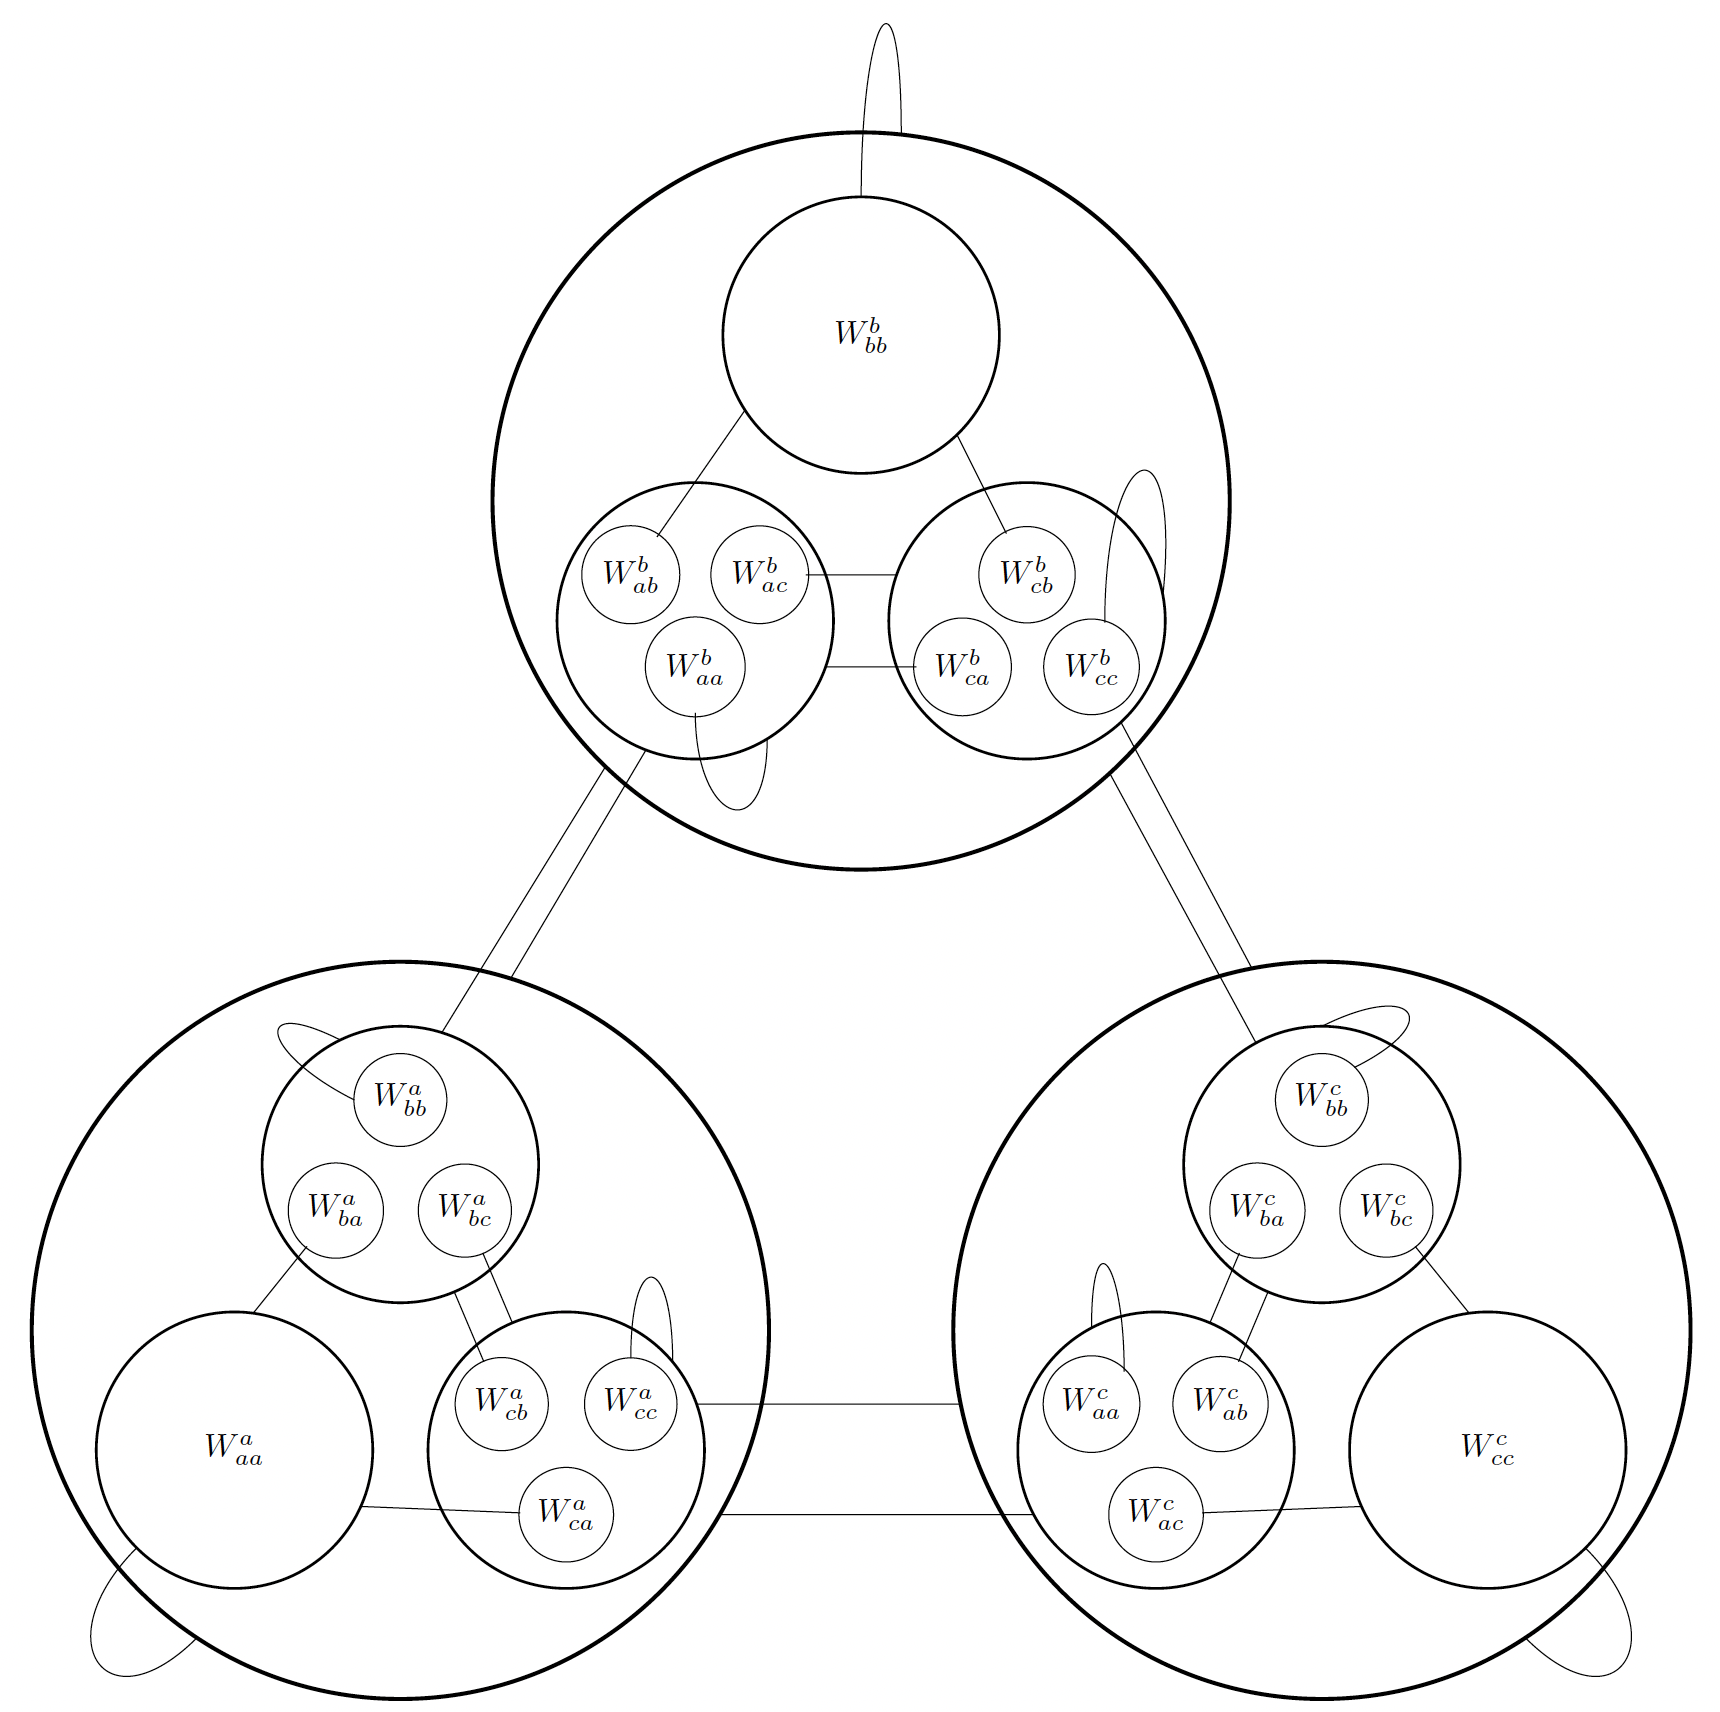
\includegraphics[keepaspectratio,width=0.7\linewidth]{../images/11_socion_tikz.png}
	\caption{階層関係を踏まえた社会関係の構造。図中の円で表現されているのが関係の重み\index[termidx]{おもみ@重み}weight要素で，上付きの添え字は保持している主体を表し，下付きの添え字はどのソシオン\index[termidx]{そしおん@ソシオン}からどのソシオン\index[termidx]{そしおん@ソシオン}への重み\index[termidx]{おもみ@重み}かを表している。すなわち，$W_{ab}^{c}$はcの考えるaからbへの重み\index[termidx]{おもみ@重み}，という意味である。}
	\label{2mode_socion}
\end{figure}

この図は非常に細かく描かれていて，記号も少しわかりにくいかもしれません。誰から誰に対する関係かというのを，Wの後の二文字で書いています。AからBに対する関係というのを，$W_{ab}$と表しています。上付きのAは，これがこのA，最初のAが誰の頭の中に入っているものかを表しています。誰の持つ，誰から誰に対する重み\index[termidx]{おもみ@重み}なのか，という書き方になっています。そしてこれが，三人からなる社会関係の全体なのではないかという提案です。

これをみながら皆さんもちょっと考えていただきたいのですが，皆さんは自我を持っていますね。自分というのが何者かというのはもちろんお分かりだと思います。そして，周りの人，周りに人がいる，あの人はこう考えているだろうな，と私が考えることができますね。あの人とあの人は，好きだろうな，嫌いだろうなという他者の関係ネットワークを推測することもできますね。その社会関係ネットワークというのを考えたときに，今言った要素が全部入っているはずです。

3人の登場人物として，この図の中にはA，B，Cがいます(大円で左下がA，中央上がB，右下がC)。ここで3人の個人と言ってしまうと物理的な境界でもって話をしているような気がするので，語弊があるかもしれませんが，太い線の大円が物理的境界であると理解してもらってもまあいいかもしれません。これが3人の社会関係，人間関係だとすると，Aさん，Bさん，Cさん，3人の人間それぞれの頭の中には，この社会関係がマルっと頭の中に入っているはずですよね。

周りを見て2人の人間がいたら，私たちは3人いるんだな，と頭の中で思うわけです。何が言いたいかというと，社会関係を1個人のシステムの内側から見ると，外側にあるだろう社会関係を頭の中にコピーしているというか，地図として持っていると言えるんじゃないか，ということです。人間関係，社会関係を。それは相互に我々持ち合っているはずです。その像が正しいかどうかは別として。

これは何が言いたいかというと，現象学的なというか，どこまで行っても，私の考える社会は，私の見ている世界は，というのから抜けられないという考えと同じです。私は今，例えばこの教室に3人の人間がいると思っています。それは知っているんですけれども，3人の人間がいると私が思っているだけなので，このAの頭の中には，私とBとCがいるでしょう。心の中のシステムとしてこういうふうになっているだろう，と描けるわけです(左下の大円の中に，全体の相似系のような三者関係が縮小されて含まれていることがそれを表しています。)。

一人の頭の中においても，例えば私はあの人のことを，あの人にこのように思われているだろうとか，この人にはこのように思われているだろうというような自覚はあります。相互にきっと何か思われているんだろう，イメージを持たれているんだろうと考えているはずなんです。私の中にある「あの人は私のことを思っているんだろうな」というのは，私が見た他者の像です。この像の中には，「あの人はあの人自身のことを」，「彼は彼自身のことを」こう考えているだろう，ということも推測として入っています。ですから，私の中に入っている他者像が，その他者自身の像を持っているだろう，とも考えられます($W_{bb}^{a}$や$W_{cc}^{a}$の箇所)。そして彼は彼女のことを，彼女は彼のことをこういうふうに思っているんじゃないかという，関係の推測もできるわけです($W_{bc}^{a}$や$W_{cb}^{a}$の箇所)。もちろん私は，自分のことをどう思っているかという自己像も持っています($W_{aa}^{a}$の箇所)。

これは一人一人の頭の中にある，社会全体の像です。自分の中に引き込んでいる他人の像というのは，よく見てみると，それはその人のイメージです。これは，私がその人のイメージを自分の中に持ち込んだものです。そして，相手もまた私の像を持っています。つまり，お互いの像を持ち合っているわけです。

この人の中から見れば，Aの人は自分自身のことをどう考えているのだろう，Bとの関係はどうなのだろう，彼は私のことをどう思っているのだろうというような関係も存在します。この部分が複雑に絡み合っていると感じる人もいるかもしれません。ただし，これでも，社会関係を考える上での最低限に絞ってるつもりです。

さて，これ($W_{aa}^{a}$)は何かと言いますと，自分が自分をどう思っているかというところです。もし，この中に複雑な要素を書き込むなら，自分が自分をどう思っているか，と思っているか，と思っているか...とか，あなたが考える私の考えるあなた，の考える私...のように，何重にも書き込むことができますね。それは，鏡を合わせたときに反射が無限に続くように，この中に無限に書き込めてしまいます。しかし，藤澤はそれは一段階で止めるべきだと言います。自分が自分をどう思っているかということは，結局自分が考えているだけで終わるべきだと。無限に続くことはないと。だからここはシンプルな絵になっています\footnote{藤澤はこれを「龍の考える麒麟」と表しています。架空の存在である龍が考える，架空の存在の麒麟は，結局龍を考えている主体の考える麒麟とおなじことである，という意味です。}。

これが，先ほどのネットワーク図をより正確に描いたものです。一般的には，私たちは社会のことを考えるときに，観察的な視点から見ます。人間関係のやり取り，例えば彼と彼女が言い争っていたとか，手をつないで歩いていたという観察可能な情報を自分の中の像として取り入れ，自分の中でその社会関係の情報を更新します。

外から見ていた，人間関係の要素だけを集めて，これが社会だということもできます\footnote{図中の$W_{ab}^{a}$のように，認識主体と重み\index[termidx]{おもみ@重み}の始点が同じ重み\index[termidx]{おもみ@重み}は，大円を飛び越えて対象と繋がっています。ここは外部に現れうる要素なので，いわゆる客観的な「人間関係の要素」ということができます。}。あるいは，一人一人に聞いていって，みんなの人間関係を全部集めてきた，その平均的なものとして，社会とか，人間関係の実態はこうだということを外から定義することもできます。

もちろん，自分の中のあなたの像を中心に考えることもできます。つまり，個人的な視点からネットワークを見るのか，外から見るのかによって，何を強調するか，どのように平均化したり一般化したりするかという違いはあるかもしれません。

ただし，基本的には，他人とのつながりという，このネットワーク図を社会的な視点から見るのか，個人的な視点から見るのかの違いにすぎません。同じ要素を持ったネットワークを個人の視点から論じるのか，社会の視点から論じるのかによって，まるで階層関係があるように見えます。

このように，階層関係というのは，同じものをどちらの視点から見ているかによるだけだと考えるのが，藤澤の階層関係の問題の解決方法です。

\section{社会心理学の本質と課題}
\subsection{社会システムの動態}
ここから考えると，これがもし正しいなら，私たちが「自分ってこんな人間なんだ」と言っているのは，存在するもの全ての中の自分の一部分だけを見ていることになります。また，「私はあの人のことをこう思いますよ」と言っているのも，その人の一部を理解しているだけに過ぎません。

社会心理学を進める上で重要なのは，個人の内側の相と外に見られる相が連動しているということです。人は「認知的不協和を解決したい」という思いをもっていたり，「他者間の人間関係がどうなっているのか」といったことを頭の中で考察し，それに基づいて行動をするわけですね。行動が一度表に出ると，その行動は社会の相に反映されます。この人が他者に対して抱いているイメージ，そしてそのイメージに基づいた振る舞いが自分の境界を超えます。それは他者に観測されるものです。

その表に出てきたものを他者が，それを基に自身の持つ情報をアップデートし，それぞれの頭の中で思考を巡らせる。そうすることで変動が引き起こされるでしょう。つまり，社会心理学で社会と心理を考える以上は，個人の内心と社会に与えた影響，そしてそれが自分のものが社会に出て，社会のものが巡り巡って自分の中に帰ってくるというダイナミクスを研究する必要があると思います。これは，自分の中だけのシステムだけで終わる話ではなく，外で見えるものだけでもないということです。

自分の中だけのシステムであればオートポエティックに自分の中だけで見るということですから，それは個人心理学です。表に見えてくる会話のパターンだけで考えるのであれば，それは社会学というか社会の話です。社会心理学というのは，自分の中と社会の状態の行き来，つまりダイナミクスを研究する必要があると私は考えています。

今の社会心理学的な研究のアプローチは，個人の中の心理学に引っ張られすぎていると感じます。また，社会に一度出したものが自分の中に返ってくるというプロセスを無視しています。自分の意見や主張，個人の社会観だけを考えている。社会関係のごく一部しか扱っていないように見えます。

皆さんは，社会心理学をどのように感じていますか？私は，現在の社会心理学は，社会学か個人心理学のどちらかにしかなっていないように感じます。本来は，個人と社会，個人と集団，集団と社会という行き来するダイナミズムを考える科学にしなければならないのではないかと思います。

ただし，これが正解だと言っているわけではありません。私は，社会心理学をこのように考えるべきだと思っていますが，皆さんなりの社会心理学というものを聞かせて欲しいんです。自分と他人の境界を行き来するもの，これが本来社会心理学で考えるべきだと私は思います。

藤澤先生も同様のことを言っており，僕も昔若い頃から藤澤先生の教えを受けているんですけど，20年くらい経ってやっと先生が言おうとしていることがちょっと分かってきたかなというところです。ひょっとしたらとんでもない勘違いをしているのかもしれませんが，システム論的に社会心理学を考えるなら，個人と社会の相互の振動，つまり相互のやりとりを中心に置いたサイエンスでないといけないだろうなというような気がします。

さて，今のところこの一つの単位が個人だという言い方をしましたけれども，この藤澤のシステム論の面白いところは，人と人とのつながり，何らかの関係性をノード\index[termidx]{のーど@ノード}にしたネットワークが，相互につながり合って広がっていくネットワークの位相空間\index[termidx]{いそうくうかん@位相空間}の中でできあがる，自己ということを考えているところです

\subsection{境界の創発と安定化}

この時のもう一つの強調すべきポイントは，物理的な実体に依存していないことです。僕というハードウェアとしての自分がなかったとしても，自分と同じような関係のパターンを持つことができるものであれば，それが自分なんです。そういう関係のパターンが成立すれば，それが一単位になるという考え方です。

個人というのは，例えば私個人というのは，僕を知る皆さんと，僕が知る皆さんと，自分で自分のことをどう捉えているか，の総体です。その関係性ネットワークの振る舞い上に現れるパターンが，実在としての私です。

ここでパターンと言う以上は，プロセスが繰り返して同じ状態に戻ってくることが大事です。同じ過程が2回以上繰り返されたことで，この関係の繋がり方，このネットワークの仕方が小杉というパターンなんだな，となるわけです。特定のパターンが動いていると，システムの完成という感じで，ソシオン\index[termidx]{そしおん@ソシオン}の境界ができるわけです。

藤澤システム論のポイントは，この境界が作られることでもってシステムが完成するという考え方です。オートポイエーシス\index[termidx]{おーとぽいえーしす@オートポイエーシス}の時の発想にだいぶん近いですね。

オートポイエーシス\index[termidx]{おーとぽいえーしす@オートポイエーシス}は，要素間の関係がぐるっと回ってパターンができたら，それがシステムだよという言い方をしました。それと同じで，このネットワークの，つながり方のネットワークのパターンが形成されたら，それが一つの社会的な単位だよと。人間個人で言うと，このわかりやすいハードウェアをフィックスするものがありますから，この界隈で起こるものという形になりますが。

例えばグループというようなことを考えてみましょう。たとえば私，自分の本務校でゼミというのを持っていますが，ゼミって一体何だろうかということを考えてみます。例えばゼミの学生というのは，この間も風邪ひいて一人休んでいたりしましたが，メンバーが欠けても，ゼミとしての活動は続くわけですね。あるいは先日うちのゼミ生が卒論書きました。彼は卒業していきますが，卒業して新しいゼミ生が入ってくると，またそこで新しいメンバーでゼミ活動というのがつながります。

つまり，ゼミシステムというのは，学生のインプットだとかアウトプットだとかがあって，物理的な部屋の中でやってる何かというものというよりは，そこの中で行われる認知的な要素，情報，関係のつながりの，こういう喋り方をしたらこういう話題になって，こういうところに話が落ち着いて，みんなが納得するというような会話のパターンだとか，人間関係のやりとり，その営みのことですよね。

会話の中身として，教師--学生のパターン，先輩--後輩のパターンなど，様々なパターンが存在します。教える--教わるパターンや，発表する--発表を聞くなどの活動のパターンが，ゼミというものです。メンバーはそのパターンを回すために存在します。「あいつがこなければゼミにならない」といった考えもあるでしょう。しかし，パターンが回る限り，例えば私がいなくてもゼミは回ることがあります。

その部屋で行われる会話を「ゼミ活動」，「そのグループ」と呼びます。毎回新しい話題，新しい形が出てくるパターンがあって，次何が起こるかがわからないとそれは一過性の人の集まり。それが1回のイベントで終わるなら，パターンを形成しません。しかし，何回か行うと，ある一定のパターンができ上がります。「仕事が回る」と言ったりしますが，あのパターンが形成される感じです。その一連の関係が回ると，ある種のパターンができ，ゼミ活動という一単位が出来上がるのです。

ネットワークのネットがワークする様子で，そのネットワークの一部が認知的，感情的な要素をつなげ，重層的になっていくんですね。何周かすると，それがどういうパターンなのかが明確になり，そのパターンが社会的な単位になります。「それ」が浮かび上がると，新たなシステムが誕生するんです。また，その境界が出来上がると，新たな単位が形成されます。「小杉ゼミってあんな感じだよね」と言えるようになります。また，「その集団はこうだね」や「ゼミのみんながお前のことを嫌ってるぞ」などと言えるようになります。そのように，一つの社会の単位として，一つの存在として機能し始めます。

このネットワークの濃度，正確には要素間の関係が要素なのですが，その一単位が創造されるところがミソです。境界が切り取られるというか，浮かび上がるというイメージ。その会話をしているときのまとまり，その会話したときのまとまりが形成されます。ネットワークの部分部分に境界が出来上がることを通じて，社会の単位が形成されます。これが藤澤システム論の面白い点だと思います。

オートポエーシスは「どこからが自己なのか」を問うことなく，全てが自己だと結論付けます。複雑系\index[termidx]{ふくざつけい@複雑系}はマクロレベルで全体のパターンが見えますが，誰が見ているのかは分かりません。藤澤システムはその境界を作り出す要素の人にとっては内側から見え，境界ができたとき含まれてない関係者にとっては外側から見えます。つまり，同じネットワークを個人のモードから見る場合と，社会のモードから見る場合があります。

同じネットワークがどこで切り上がって，内側になったのか，外側になったのかは，その状況によります。これはオートポエーシスが言う相互浸透ではなく，カップリング\index[termidx]{かっぷりんぐ@カップリング}の仕方です。切り取られたシステムの内側から見る場合，外側から見る場合，自己というのを含んでいるシステム，自己を含んでいるシステムとなります。

要素，つまり関係のパターンが新しいシステムになりますよというところが，この藤澤システム論の面白いところかなと思います。社会の単位というのを考える。この社会の単位というのは，関係のパターンが出来上がった時に，境界の部分だけ切り出されて出来上がってくるもの。これが，複合システムネットワーク\index[termidx]{ふくごうしすてむねっとわーく@複合システムネットワーク}論で言うところのネットワークの単位。その単位が変数が出来上がるとか，消えるっていうような話っていうのは，今までのシステム論ではなかった話です。

ベルタランフィ\index[nameidx]{べるたらんふぃ@ベルタランフィ}のシステムは，連立微分法程式でしたから，全てのシステムの要素を外的に固定して書いていました。複雑系\index[termidx]{ふくざつけい@複雑系}は，近傍との関わりは書いたとしても全体を見ているところを書いていませんでした。オートポイエーシス\index[termidx]{おーとぽいえーしす@オートポイエーシス}は数学的な表現をしていないし，藤澤システム論も数式的な表現は出来ていないのですが，これらを考えるヒントにはなっていると思います。

\subsection{社会関係のマトリクス}

このネットワーク関係みたいなのは，グラフ理論もそうですが，図で表現しているのが今の書き方です。しかしこれは行列で表現することも出来ます。例えば，A，B，Cという3つのネットワークがあって，AがCと繋がっている，AがBと繋がっている，BとCは繋がっていないというパターンがあった時，これを行列だと，「AはBと繋がっている，AはCと繋がっている，BはCと繋がっていない」と書くことができます。繋がっていれば1，繋がっていなければ0となります(図 \ref{matrix_expression})。
\begin{figure}[ht]
	\centering
	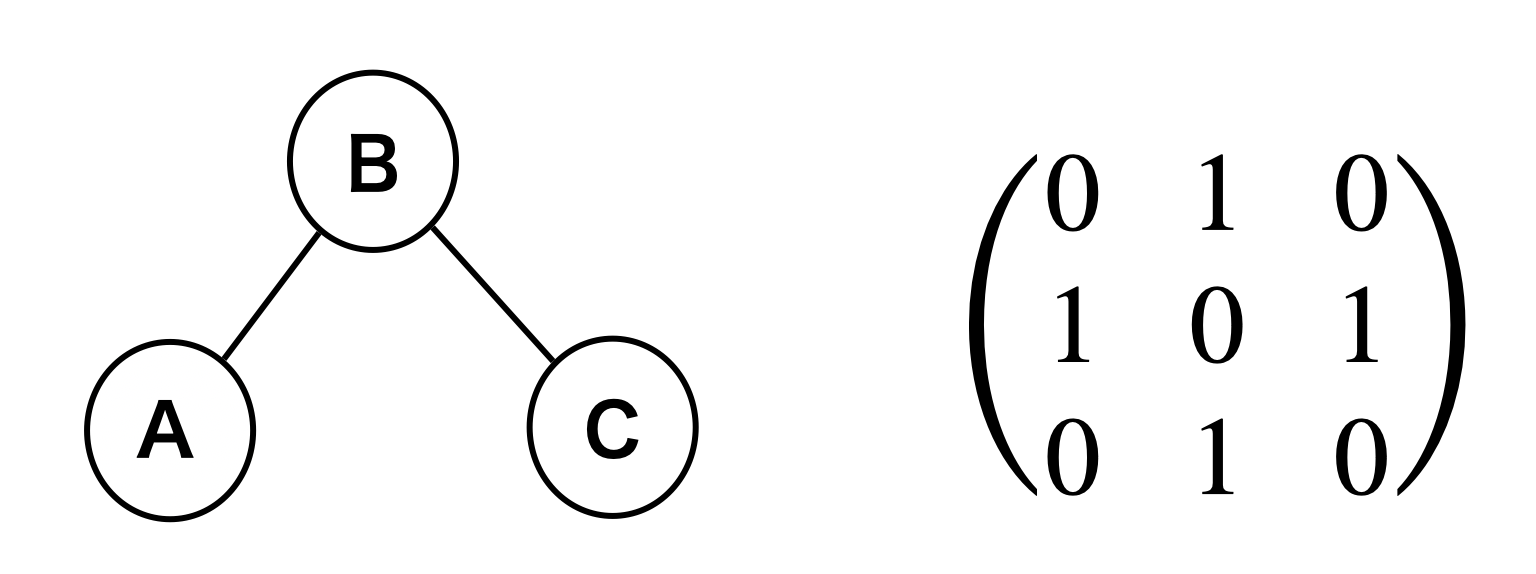
\includegraphics[keepaspectratio,width=0.7\linewidth]{../images/11_matrix.png}
	\caption{グラフ表現と行列表現の相同性}
	\label{matrix_expression}
\end{figure}

また，このようなネットワークを行列のような形で書くことが出来ます。グラフの表現は，この行列の書き方と同じです。これを拡張して，藤澤システム流に考えてみましょう。

私が考える私，私が考える他者，A，B，C，などがあります。
私が考える私を「自己」という風に言い，私が考える他者を「対人的態度」という風に言うことが多いです。同じく，他者A，B，Cに対し，相手から見た自分の像，つまり「他己」もあります。社会心理学において，ここを考えていることは少ないかな，と思います。

さて，社会心理学でアンケート調査をする時，「自分の相手のことをどう思いますか」「あなたは周りにどう思われていますか」「あなたはどのように考えていますか」と聞くことがありますが，ここ(関係の推測)の部分はあまり聞かないですよね。
\begin{figure}[ht]
	\centering
	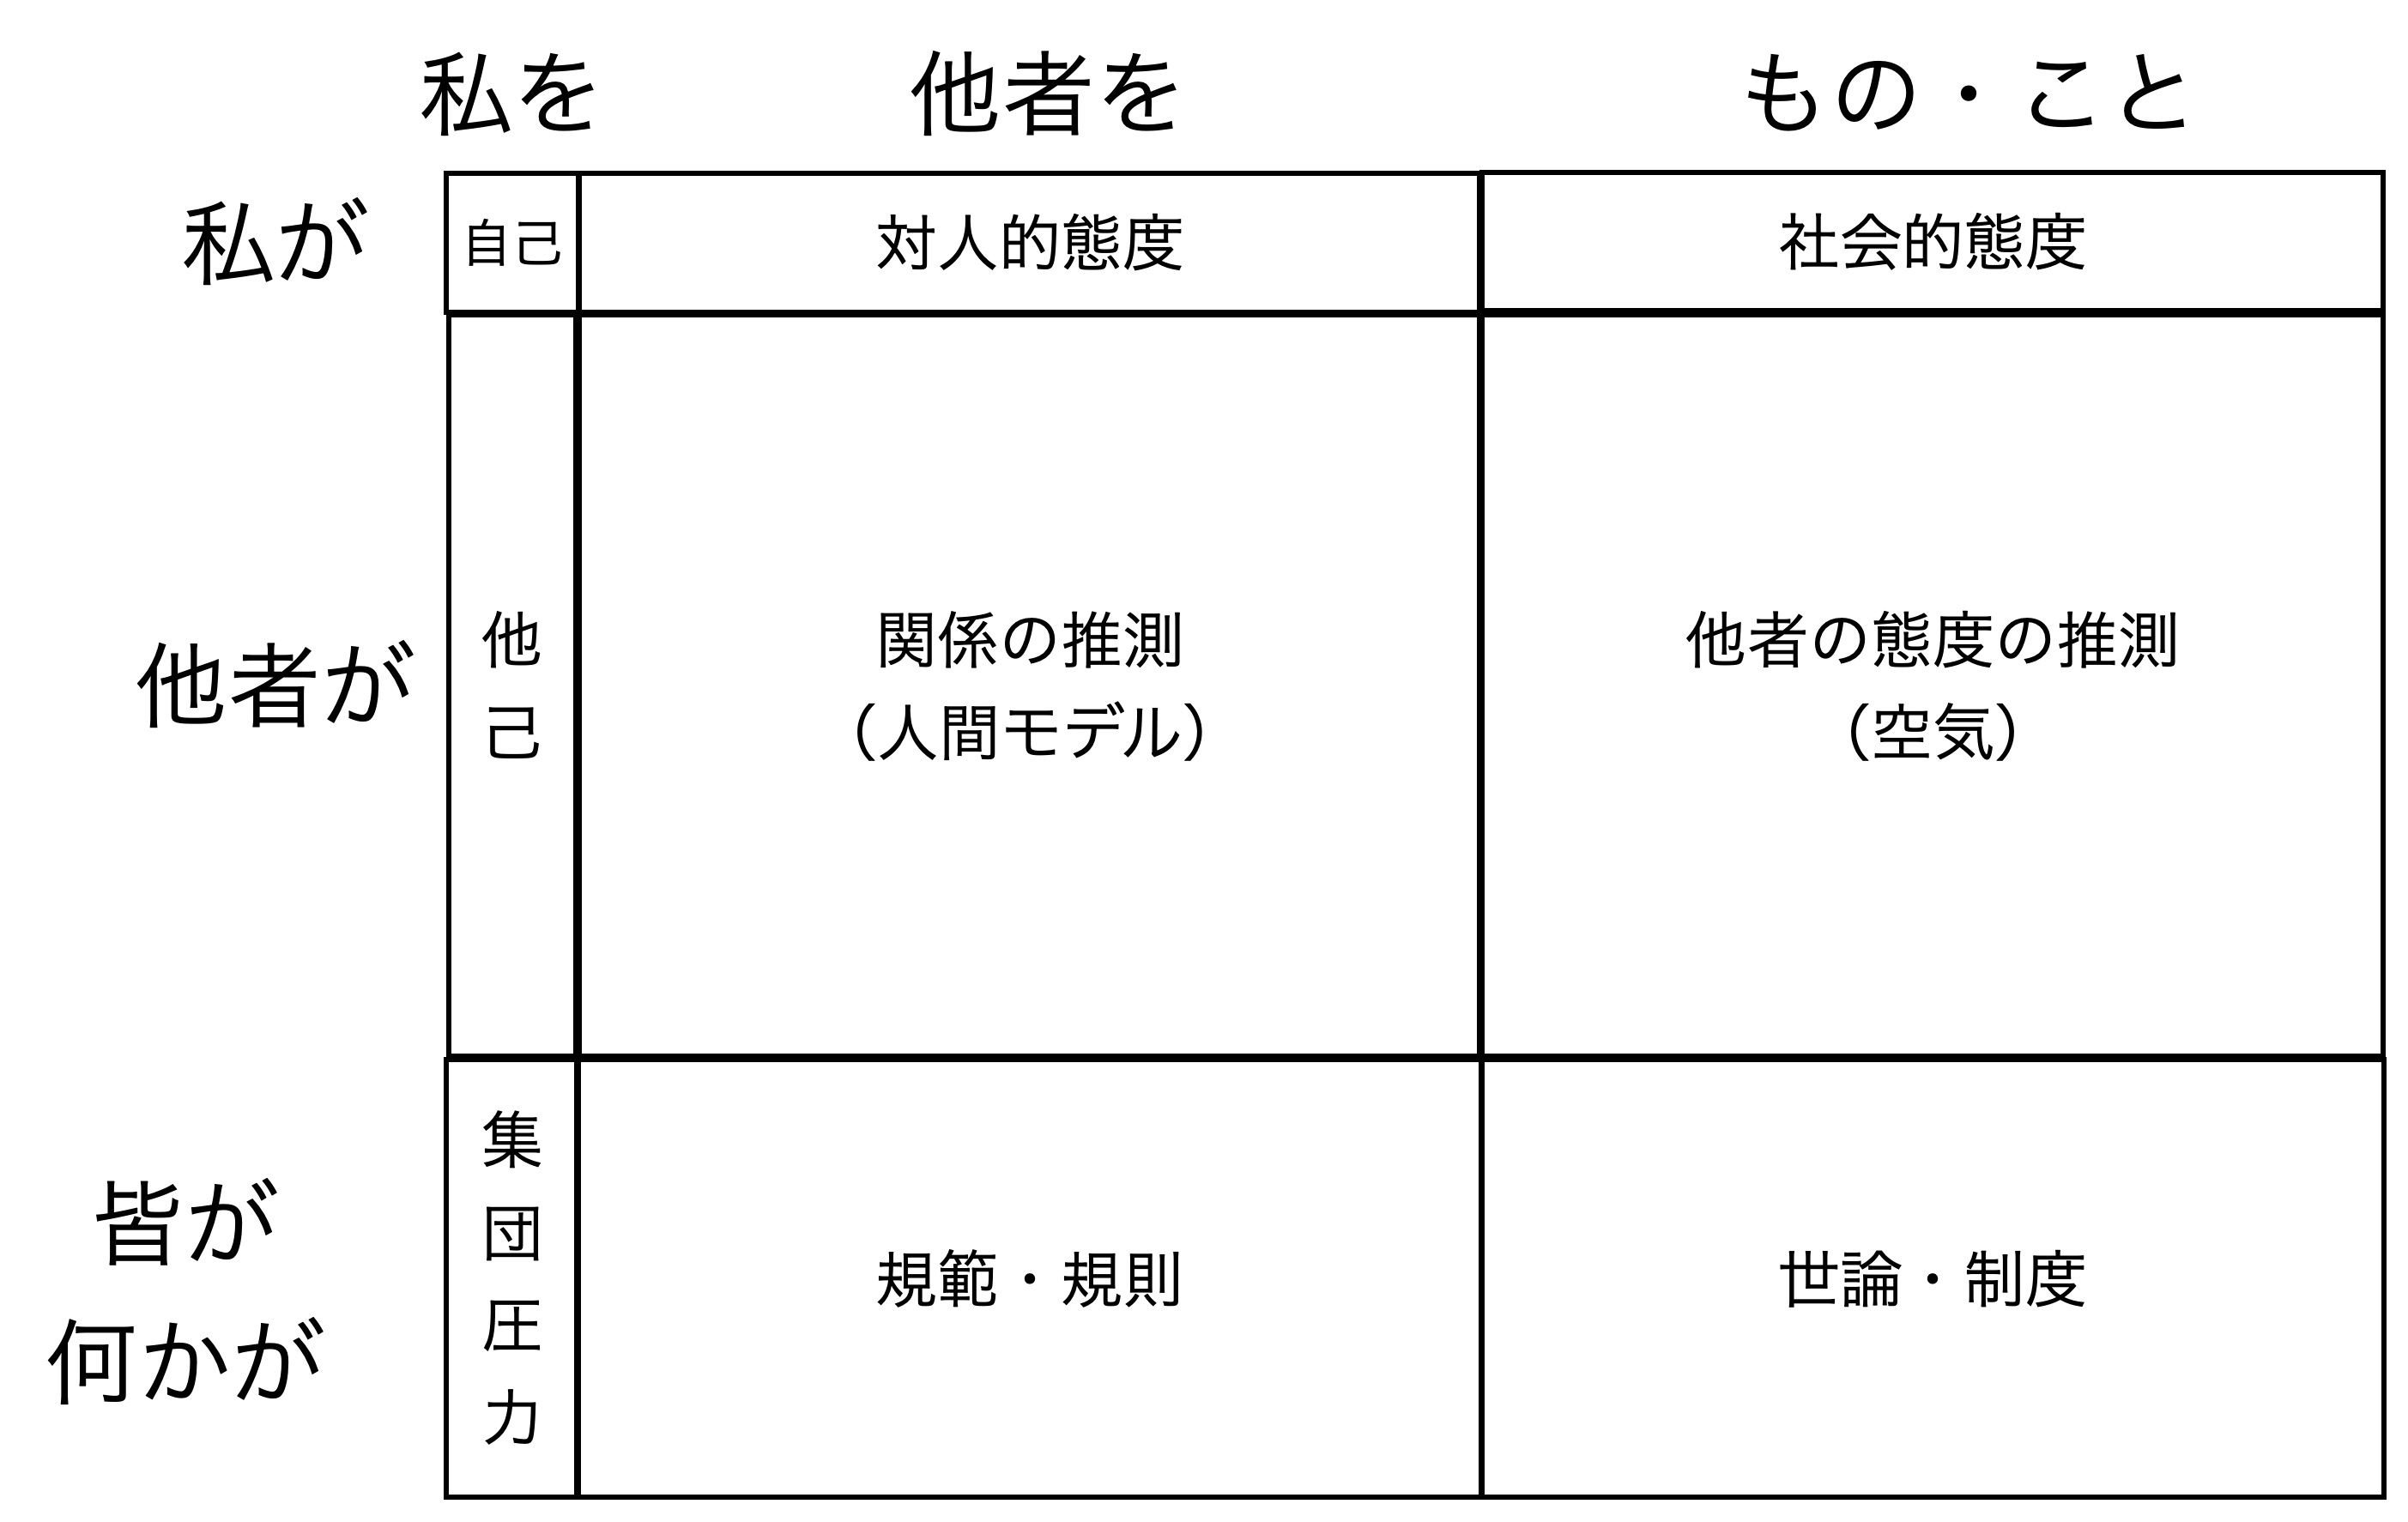
\includegraphics[keepaspectratio,width=0.7\linewidth]{../images/11_expanded_matrix.png}
	\caption{拡張された関係行列}
	\label{expanded_matrix_expression}
\end{figure}

これは，他者関係の推測になっているわけですが，僕はもっとこの部分を研究するべきだと思います。他人が考えている他人ですから，自分のことではないかもしれませんが，自分の中に入っている社会的な要素であることは間違いないです。その他者に対する他人の人間関係も少なからず自分に影響しているはずです。

この辺の要素・領域は非常に広いはずですが，測定しにくいということもあるのかもしれません。そのため，あまり評価されていないのかもしれません。

さて，この行列には他の要素もあります。社会的な対象，社会的な実在，これらに関しても社会心理学がありますね。これは何かというと，社会的な態度と一般的に言われます。次回やるつもりですが，社会的態度\index[termidx]{しゃかいてきたいど@社会的態度}の研究というのはここの部分です。自民党に対する態度だとか，環境破壊問題に対する態度など。自分は社会のイシューに対して，このようなことを考えていますという類のものです。
これに対して，他者による態度，すなわち推測された社会的な態度という領域もあります。「あの人はきっとこういう態度を持っているだろう」という部分です。

同じように，社会的な実在が自分に対してどのようなことを言ってくるか，みんなが私のことをどう思っているかとか，日本人というのはどう思われているかというような部分もあるでしょう。それはみんなが私をどう思うか，という点では集団圧力ですし，みんなが他者をどう思っているか，という点で集団規範，規則の話です。他の人が考えている，このゼミにおける雰囲気的な側面などです。「あいつのところがこんなになってそうだな」というような感じです。最後に，みんなが考えている社会的実在\index[termidx]{しゃかいてきじつざい@社会的実在}に対する評価，これが世論とか制度と呼ばれるものですね。

社会的な実在と人間をこのように行列で考えたときに，一人の頭の中にこんなにもの要素があるはずです。これは一人の頭の中であり，全てが一個人の考えです。そして，この行列が各人の中にありますので，社会心理学はその総体を研究することになります。

社会心理学が考えなければいけない要素は非常に大きいですが，実際に研究されているのは，せいぜい自己と対人的態度，社会的態度\index[termidx]{しゃかいてきたいど@社会的態度}ぐらいだと思います。まだまだ考えないといけない部分は残っており，しかもその自分の考える全体とか，階層を変えたときの自己と社会，自分と集団，集団と社会などの関係も，本来は社会心理学の研究テーマになるはずです。

廣田君美\index[nameidx]{ひろたきみよし@廣田君美}が「集団の心理学」\parencite{HirotaKimiyoshi}というものを書いたとき，すでにシステムの階層について言及していました。集団の研究というのはシステム全体だけでなく，サブシステム，サブサブシステム，サブグループ，サブサブグループも含まれます。人間は10人集まったらサブグループができると言いますが，10人集まったらサブグループがあり，サブグループと全体との関係，例えば学級の中の各班と学級全体との関係，自分と班との関係，自分と学級との関係，全て頭の中で社会関係を計算しながら，その辺をいろいろ考えて行動するわけです。

なので，本来はこのような階層的な関係，入れ子になっている階層的な関係を全部考えないといけないんですけど，社会心理学はその中でもごくごく一部の「自分が評価する」という，このマトリクスの第一行に限って研究をしているかのようです。この部分が現代社会心理学の不完全さではないかと僕は思っていますが，いかがでしょうか。

\section{社会心理学の展望と課題}
\subsection{第五世代システムのまとめ}
藤澤のシステム論について最後にまとめますと，社会の構成単位は複合システム\index[termidx]{ふくごうしすてむ@複合システム}であり，それらは互いに影響し合う重み\index[termidx]{おもみ@重み}を持っています。これらの単位は最初から入れ子状に組み込まれており，そうしたネットワークの単位とその動きを体系化したものが彼の理論です。

この理論の興味深い点は，こうした単位の概念を確立したことと，それに基づく社会の動きについての仮説を提示したことです。しかし，先ほども強調したように，最も重要なのは，これらの単位を区切るシステムの境界線が，ネットワークの相互作用によって自然に生まれてくるという考え方です。つまり，境界が自然発生的に現れるという現象が，この理論の核心なのです。

オートポイエーシス\index[termidx]{おーとぽいえーしす@オートポイエーシス}という考え方が「自己」が生まれることに着目したのに対し，藤澤の理論はより広く「境界」が生まれることに注目しました。この境界の形成は，ネットワークの結節点が増えることであり，同時に「ソシオン\index[termidx]{そしおん@ソシオン}」という新しい社会単位が増えることでもあります。

ただし，この現象を具体的に表現することは非常に困難です。数学の計算では変数が途中で増減することはありますが，プログラミングやシミュレーションでは，途中でエージェント(作用する主体)が増減する動的な配列を作るのは技術的に難しいのです。例えば，セルオートマトン\index[termidx]{せるおーとまとん@セルオートマトン}では，最初にサイズを決めます。もしセルの数が途中で増減すると，その都度メモリや描画領域を割り当て直す必要があり，非常に複雑な処理が必要になります。実際，以前に知人とJavaでそのようなプログラムを書こうとしましたが，処理が複雑すぎてコンピュータがフリーズしてしまい，実用的なものは作れませんでした。今の言語，PCスペックならできるかもしれませんが。

この授業で以前も説明しましたが，社会的な実在(社会の中で実際に存在するもの)というのは，人々がそれを「確かにある」と認識すれば生まれ，逆に人々がその存在を忘れてしまえば消えていくという特徴があります。

これは社会的なものの本質的な性質です。つまり，社会的なものは生まれたり消えたりするのです。それはつまり，境界線が生まれたり消えたりているということです。そして，システムを構成する要素も，この境界の創発\index[termidx]{そうはつ@創発}と消失に応じて増えたり減ったりするのです。

この要素の増減は，システム自体の挙動によって決まってきます。藤澤のシステム論が画期的だったのは，このような説明の仕方をしたところにあります。
\subsection{階層間関係の仮説}

また藤澤のシステム論では，システムの目的は「パターンの形成とその安定化」にあるとされています。それぞれの世代のシステムにおいて，この目的は異なる形で現れます。第一世代システム\index[termidx]{だいいちせだいしすてむ@第一世代システム}では動的な安定を達成すること，第二世代システム\index[termidx]{だいにせだいしすてむ@第二世代システム}ではマクロレベルでの安定を実現すること，第三世代システム\index[termidx]{だいさんせだいしすてむ@第三世代システム}では自己の世界を確立すること，そして第四世代システム\index[termidx]{だいよんせだいしすてむ@第四世代システム}では自己増殖・再生するパターンを生み出すことが目的とされています。そして，社会心理ネットワークや複合システムネットワーク\index[termidx]{ふくごうしすてむねっとわーく@複合システムネットワーク}では，パターンの維持・安定そのものが目的となります。

ただし，ここで話が複雑になるのは，社会の目的と個人の目的は，実は同じものを異なる視点から見ているに過ぎないという点です。そして，「パターンを維持すること」が本当に目的として適切なのかどうかを，実際に確かめることは難しいのです。

一応その目的が正しいとしましょう。社会は社会として安定を求めて動き，個人も個人として安定を求めて動きます。その際，社会と個人は互いに影響を及ぼし合いながら存在しています。個人と社会は相互に作用しながら，それぞれの安定を目指します。個人の内面が安定すれば，それは社会の安定にもつながるのかもしれません。

繰り返しますが，個人の心の中のロジックも，社会の側のロジックも，どちらもがそれぞれの安定状態を目指して動いている，というのが藤澤システム論の目的関数ですね。そして個人と社会は同じネットワークを見る視点の違いに過ぎない，ということでした。となると同じネットワークでも，社会の視点から見るか個人の視点から見るかで，安定の形は異なっているかもしれません。

どうも藤澤先生は，社会の目的関数と個人の目的関数，つまり社会が安定しようとすることと個人が安定しようとすることは，相反する結果になりがちだと考えているようです。それが本当か，正しい洞察かどうかについては，私はもう少し考えてみないといけないなと思ってます。

例えば，藤澤先生の研究には「家族システム」に関するものがあります。家族システムの研究が面白いところは，家族全体が安定しようとするとき，各人がちょっとずつ自分のワガママを我慢しなければならない，ということにあります。その結果，個人システムは少し不安定になるかもしれません。しかし，それぞれが少し我慢することで，家族全体は円満になるのです。逆に，各人が自分のワガママを優先すると，家族全体としての一体感が失われる。社会全体としては安定が損なわれるのです。

藤澤研では，これをテーマにした研究が行われました。そこでは例えば，5人家族では個々の幸福度は低いですが，全体としての幸福度が高い。一方，3人家族では個々の幸福度は高いけれど，全体としての幸福度は低いといった結果報告されています\footnote{本来，ここで論文などを引用すべきですが，明確にこの相反関係を示したものが出ていないようです。}。

藤澤システムでは，社会が頑張れば個人が不幸になるし，個人が頑張れば社会のシステムが不安定になる。これは対立構造として考えることができます。しかし，これがシステムの真の姿かどうかは，必ずしも明らかではありません。階層ごとの目的が相反するのかどうか，同じネットワークを社会の側から見たときと個人の側から見たときで，安定状態が相反するのかどうか。これらについては，まだ議論が足りないと思います。皆さんも考えてみてください。

\section{第五世代システム論からみた社会心理学}

さて，今日は藤澤先生の本\parencite{fujisawaNetwork}を中心に話を進めてきました。彼の考えは，社会心理学界では30年近く前から主張されてきましたが，それが広く受け入れられているとは必ずしも言えません。ただ，僕がこれまで話してきた社会心理学の歴史や，システム論の系譜から考えると，社会心理学はどのような学問であるべきかをテーマにした時に，非常に示唆的な観点があって，社会心理学をシステム論の観点から見ることは重要だろう，とは思います。

皆さんには，社会心理学とはどういう学問かを考えてもらいたいと思います。これまでの授業で，そのためのヒントを提供してきたつもりです。なので，その点について考えて，最終的な課題として提出してもらいたいと思います。

その前に，今のところ僕が考えている社会心理学の姿がどうであるか，ということを示しておかないと，少しズルい気がするので，ちょっとまとめておきます。決してこれが正解とか，この方向性で課題を書きなさいと言ってるわけではないので，そこはご注意ください。

私が考える社会心理学は，「2つの相(内外，自己と他者，個人と社会，集団と社会)が交錯する場面において，より共通了解の程度が高い物語を共有・強化・汎化する試み」です。

例えば個人と社会，あるいは個人と集団，集団と社会，個人と社会，または自己と他者といった，少なくとも二つの相，自他二つのシステムが，どう関係しているか。どのように交錯するか，ということをテーマにして，それらがどのように交わっているのかを考えるための学問が，僕が考える「社会心理学の本質的な問い」です。

言い方を変えると，個人の心の中だけで完結している，あるいは社会の側だけの観点で完結している社会心理学は不完全なのではないかと思っています。人間はどうやっても個人の中の世界を飛び越えることはできませんが，調査法や実験法などを用いて複数の人間を扱い，その全体に対して「全体はこうなっています」という情報をフィードバックすることで，個人と全体，個人と他者，これら2つのシステムの行き来ややり取りを研究するのが社会心理学だと考えています。

それがなければ，社会心理学は不要だとも思います。個の心理学だけで良いのです。または，社会的な刺激に反応する個人心理学とでも言えば良いと思います。社会心理学という限りは，個人のシステムと，個人でない他のシステムとのインタラクションがなければ不十分だと思います。更に言うと，個人が他者に影響を与え，その影響が回り回って自分にどう影響を与えたか，またそのことによって次の出力がどうなったかといったことを研究しなければなりません。一方通行だけでは，ネットワークにはなれないからです。ただの情報の伝達だけではなく，全体の挙動が変わるといったことを研究するのが，社会心理学であるべきだと思っているわけです。したがって，2つの相が交錯する場面において，どういう流れがあるかということを，皆で共有するための理論が社会心理学なんじゃないか。

語尾に，共有するといった言い方をしましたが，これがサイエンスかと言われると，一応これもサイエンスだ，と思います。科学とは何かという話もしてきました。科学とは，共通で理解でき，納得できる程度が高い説明原理だと思っています。したがって，2つの相が交錯する場面において，共通理解が高い物語を共有したり，その物語を一般化することが，社会心理学の役割であろうと考えています。

私の定義する社会心理学は，そんな感じです。皆さんにとっての社会心理学がどういうものであるのか，それを考えるきっかけになればいいと思い，今のような話をしています。長々と話しましたが，皆さんに何か考える素材を提供できていれば，それだけで満足です。ただ，私の言っていることが理解できなかったと思うかもしれません。自分でも抽象度が高い話を延々としていますので，うまく伝えられているかどうかわかりません。しかし，皆さんに色々考えるヒントを提供するつもりで，紹介した本を読みながら考えてみてください。

次回の授業では，現代社会心理学への批判的な検討を行います。具体的には，現代社会心理学で最も一般的に使われている調査研究の方法や分析モデルを取り上げ，それらの問題点を指摘していきます。
私が考える本来あるべき社会心理学の姿と照らし合わせると，現在の研究実践には大きな隔たりがあります。社会心理学の概念が誤って使われている例や，現在の社会心理学に不足している視点，そして方法論上の問題点などについて具体的に説明します。
つまり，「このようなやり方では不適切である」という観点から，現代の社会心理学を批判的に検討することで，この授業のまとめとしたいと思います。

シラバスにはパート3として，方法論的な問題点の指摘という話をしておりましたが，それを最後の一回でしてみたいと思います。

はい，長々と喋ってまいりましたが，今日の話はここまでにしましょう。皆さん，お疲れ様でした。


\end{document}

